\section{Farmaci del sistema respiratorio}

\subsection{Asma}

\begin{tikzpicture}
	\tikzset{level 2/.style={level distance=130pt}}
	\tikzset{level 3/.style={level distance=130pt}}
	\Tree
	[.Asma
		[.{malattia infiammatoria\\ delle vie aeree}
			{infiammazione}
			[.{ostruzione bronchiale}
				{solitamente reversibile}
				{in alcuni casi irreversibile}
			]
			{iperreattività agli allergeni}
		]
	]	
\end{tikzpicture}

\begin{tikzpicture}
	\Tree
	[.sintomi
		{sibili respiratori}
		{dispnea}
		tosse
		{costrizione torace}
	]
\end{tikzpicture}

\begin{tikzpicture}
	\tikzset{level distance=80pt}
	\Tree
	[.fisiopatogenesi
		[.{ingesso allergene}
			[.{APC presentano\\ antigeni ai \ce{T_H_2}}
				[.{\ce{T_H_2} stimolano B\\ a produrre IgE}
					[.{IgE si legano\\ agli allergeni}
						\node[dummyc]{};
					]
				]
			]
		]
	]
	\begin{scope}[yshift=-4em]
	\Tree
	[.\node[dummyc]{};
		[.{Mastociti legano IgE}
			{fase immediata}
			{fase tardiva}
		]
	]
	\end{scope}
\end{tikzpicture}

\begin{tikzpicture}
	\tikzset{level 1/.style={level distance=75pt}}
	\tikzset{level 2/.style={level distance=90pt}}
	\tikzset{level 3/.style={level distance=90pt}}
	\tikzset{level 4/.style={level distance=80pt}}
	\Tree
	[.{fase immediata}
		[.{mastociti\\ liberano}
			[.istamina
				[.{liberazione \ce{Ca^2+} nel REL}
					{broncospasmo}
				]
			]
			[.{leucotreni/citochina}
				[.IL5
					[.{attivazione eosinofili}
						{danno tissutale}
						{edema}
						{congestione}
					]
					[.{fase tardiva}
					]
				]
				[.IL4
					{stimolo a produrre IgE}
				]
			]
			[.{fattori di crescita}
			]
		]
	]
\end{tikzpicture}

\begin{tikzpicture}
	\tikzset{level distance=140pt}
	\Tree
	[.{fase tardiva}
		{inspessimento della parete\\ con restringimento del lume}
		{flogosi}
		rimodellamento
		{$\uparrow$produzione muco}
	]
\end{tikzpicture}

tutto ciò causa iperresponsività bronchiale futura.

\begin{tikzpicture}
	\tikzset{level distance=140pt}
	\Tree
	[.{farmaci}
		[.{broncodilatatori\\ (a breve durata d'azione)}
		]
		[.{glucocorticosteroidi\\ (in aerosol)}
		]
		[.{broncodilatatori\\(a lunga durata d'azione)}
		]
		[.{metilxantine o\\ antagonisti dei leucotreni}
		]
		[.{corticosteroidi orali}
		]
		[.{anticorpi monoclonali anti--IgE}
		]
	]
	\begin{scope}[xshift=18em]
		\draw[drawarrow] (0,2) -> (0,-2);
		\node[text width=8em] at (2,0){step operativi via via che la malattia diventa più grave};
	\end{scope}
\end{tikzpicture}

\begin{tikzpicture}
	\tikzset{level 1/.style={level distance=150pt}}
	\Tree
	[.{broncodilatatori}
		[.{$\beta_2$--agonisti\\(1a linea)}
			[.{a breve durata}
				\node[farmaco]{\index{salbutamolo}salbutamolo};
				\node[farmaco]{\index{terbutalina}terbutalina};
			]
			[.{a lunga durata}
				\node[farmaco](sal){\index{salmeterolo}salmeterolo};
				\node[farmaco](for){\index{formoterolo}formoterolo};
			]
		]
		[.{metilxantine\\(2a linea)}
			\node[farmaco]{\index{teofillina}teofillina};
			\node[farmaco]{\index{teobromina}teobromina	(cioccolato)};
			{caffeina};
		]
		[.{antagonisti muscarinici\\ (raramente usato. Più per BPCO)}
			\node[farmaco]{\index{ipratropio}ipratropio};
			\node[farmaco]{\index{tiotropio}tiotropio};
		]
	]
\end{tikzpicture}


\begin{tikzpicture}
	\Tree
	[.{$\beta_2$--agonisti}
		[.meccanismo
			{stimolazione $\beta_2$ muscolo bronchiale\\ con dilatazione}
			{inibizione del rilascio\\ dei mediatori dai mastociti}
			{$\downarrow$essudato}
		]
		[.somministrazione
			{inalazione per evitare\\ effetti sistemici}
		]
		[.metabolismo
			{epatico/renale}
		]
		[.{effetti collaterali}
			tachicardia
			{tremore muscolare}
		]
	]
\end{tikzpicture}

\begin{tikzpicture}
	\tikzset{level 2/.style={level distance=150pt}}
	\Tree
	[.{metilxantine}
		[.meccanismo
			{inibizione fosfodiesterasi IV (PDE)\\ che degrada cAMP quindi\\$\uparrow$cAMP$\Rightarrow$miorilassamento$\Rightarrow$broncodilatazione}
		]
		[.somministrazione
			os
		]
		[.metabolismo
			{epatico P450/renale}
		]
		[.{effetti collaterali}
			tachicardia
			{tremore muscolare}
			insonnia
			{$\uparrow$motilità intestinale}
		]
	]
\end{tikzpicture}

\begin{tikzpicture}
	\Tree
	[.{glucocorticoidi\\(GC)}
		\node[farmaco]{\index{idrocortisone}idrocortisone\\(EV)};
		\node[farmaco]{\index{beclometasone}beclometasone\\(aerosol)};
		\node[farmaco]{\index{budesonide}budesonide\\(aerosol)};
	]
\end{tikzpicture}

\begin{tikzpicture}
	\tikzset{level 2/.style={level distance=150pt}}
	\Tree
	[.{glucocorticoidi\\(GC)}
		[.meccanismo
			{$\downarrow$citochne}
			{inibizione COX2$\Rightarrow$inibizione\\ eosinofili e basofili}
			{inibizione leucotreni}
			{$\downarrow$edema}
			{$\uparrow$recettori $\beta_2$}
		]
		[.somministrazione
			{aerosol/EV}
		]
		[.{effetti collaterali}
			{sindrome di Cushing}
			disfonia
			{candidosi orofaringea\\(mughetto)}
		]
	]
\end{tikzpicture}

I GC vengono dati alle partorienti con figlio prematuro per velocizzare la funzione del surfactante polmonare che innalza la tensione degli alveoli e evita il collasso polmonare.

\begin{tikzpicture}
	\Tree
	[.{inibitori di\\ rilascio dei mediatori}
		[.\node[farmaco]{\index{cromolin}cromolin};
			[.meccanismo
				{inibizione del rilascio\\ di leucotreni e istamina\\ dai mastociti}
			]
			[.somministrazione
				{aerosol via\\ inalatori nasali}
			]
			[.{indicazioni terapeutiche}
				{allergie alimentari}
				{riniti allergiche}
				{congiuntiviti}
				{asma (raro utilizzo)}
			]
		]
	] 
\end{tikzpicture}

\begin{tikzpicture}
	\tikzset{level 1/.style={level distance=130pt}}
	\tikzset{level 2/.style={level distance=130pt}}
	\Tree
	[.{antagonisti dei leucotreni}
		[.meccanismo
			[.{bloccanti dei recettori\\ per i leucotreni}
				\node[farmaco]{\index{zafilukast}zafilukast};
				\node[farmaco]{\index{montelukast}montelukast};
			]
			[.{inibitori della lipossigenasi}
				\node[farmaco]{\index{zileuton}zileuton};
			]
		]
		[.somministrazione
			os
		]
		[.{indicazioni terapeutiche}
			{broncospasmo da antigene,\\ esercizio fisico o aspirina}
		]
		[.{effetti collaterali}
			{vasculite sistemica (leucotreni)}
			{$\uparrow$transaminasi (lipossigenasi)}
		]
	]
\end{tikzpicture}

\begin{tikzpicture}
	\Tree
	[.{anticorpo monoclonale\\ anti--IgE}
		[.\node[farmaco]{\index{omalizumab}omalizumab};
			[.somministrazione EV
			]
			[.difetti costoso
			]
		]
	]
\end{tikzpicture}

\newpage